\chapter{General Framework of the Project}
\minitoc
\clearpage
\section{General Context of the Project}
This chapter introduces the organizational context of the internship, explains the problem addressed by the project, presents the main system requirements, and justifies the development methodology that was adopted.

\section{Company Presentation}
This internship was carried out at \textbf{OneTech Business Solutions (OTBS)}. OTBS is part of the OneTech Group and belongs to its ICT activity area \cite{otbs-website,otbs-linkedin}. The company specializes in technology integration and IT solutions for business clients. Since several teams often work on different projects at the same time, day-to-day coordination depends heavily on reliable digital tools.

Within the HR and project follow-up workflow, two internal systems were already in use: \textbf{BioTime} for attendance tracking and \textbf{EasyProject} for HR and project-related data. Although each system functioned correctly on its own, they were not directly synchronized.

\begin{center}
	\renewcommand{\arraystretch}{1.2}
	\begin{tabular}{|l|>{\raggedright\arraybackslash}p{10cm}|}
		\hline
		\textbf{Company} & OneTech Business Solutions (OTBS) \\
		\hline
		\textbf{Industry} & ICT / IT integration services \\
		\hline
		\textbf{Group Affiliation} & Subsidiary of OneTech Group (ICT activity) \\
		\hline
		\textbf{Business Focus} & Integration and distribution of information and communication technologies (ICT) \\
		\hline
		\textbf{Existing Systems} & BioTime (ZKTeco biometric attendance) + EasyProject (project \& HR management) \\
		\hline
		\textbf{Infrastructure} & On-premise PostgreSQL and MySQL databases, internal network \\
		\hline
		\textbf{Internship Duration} & 3 months (approximately 12 weeks) \\
		\hline
		\textbf{Intern Role} & Full-Stack Developer --- Design, ETL, Backend (FastAPI), Frontend (React) \\
		\hline
	\end{tabular}
\end{center}

\subsection{Organizational Chart}
The organizational chart in Figure~\ref{fig:group-management-structure} presents the group management structure of the company and highlights its position within the broader organizational hierarchy.

\clearpage
\thispagestyle{plain}
\begin{figure}[p]
	\centering
	\IfFileExists{logos/organizational-chart.pdf}{%
		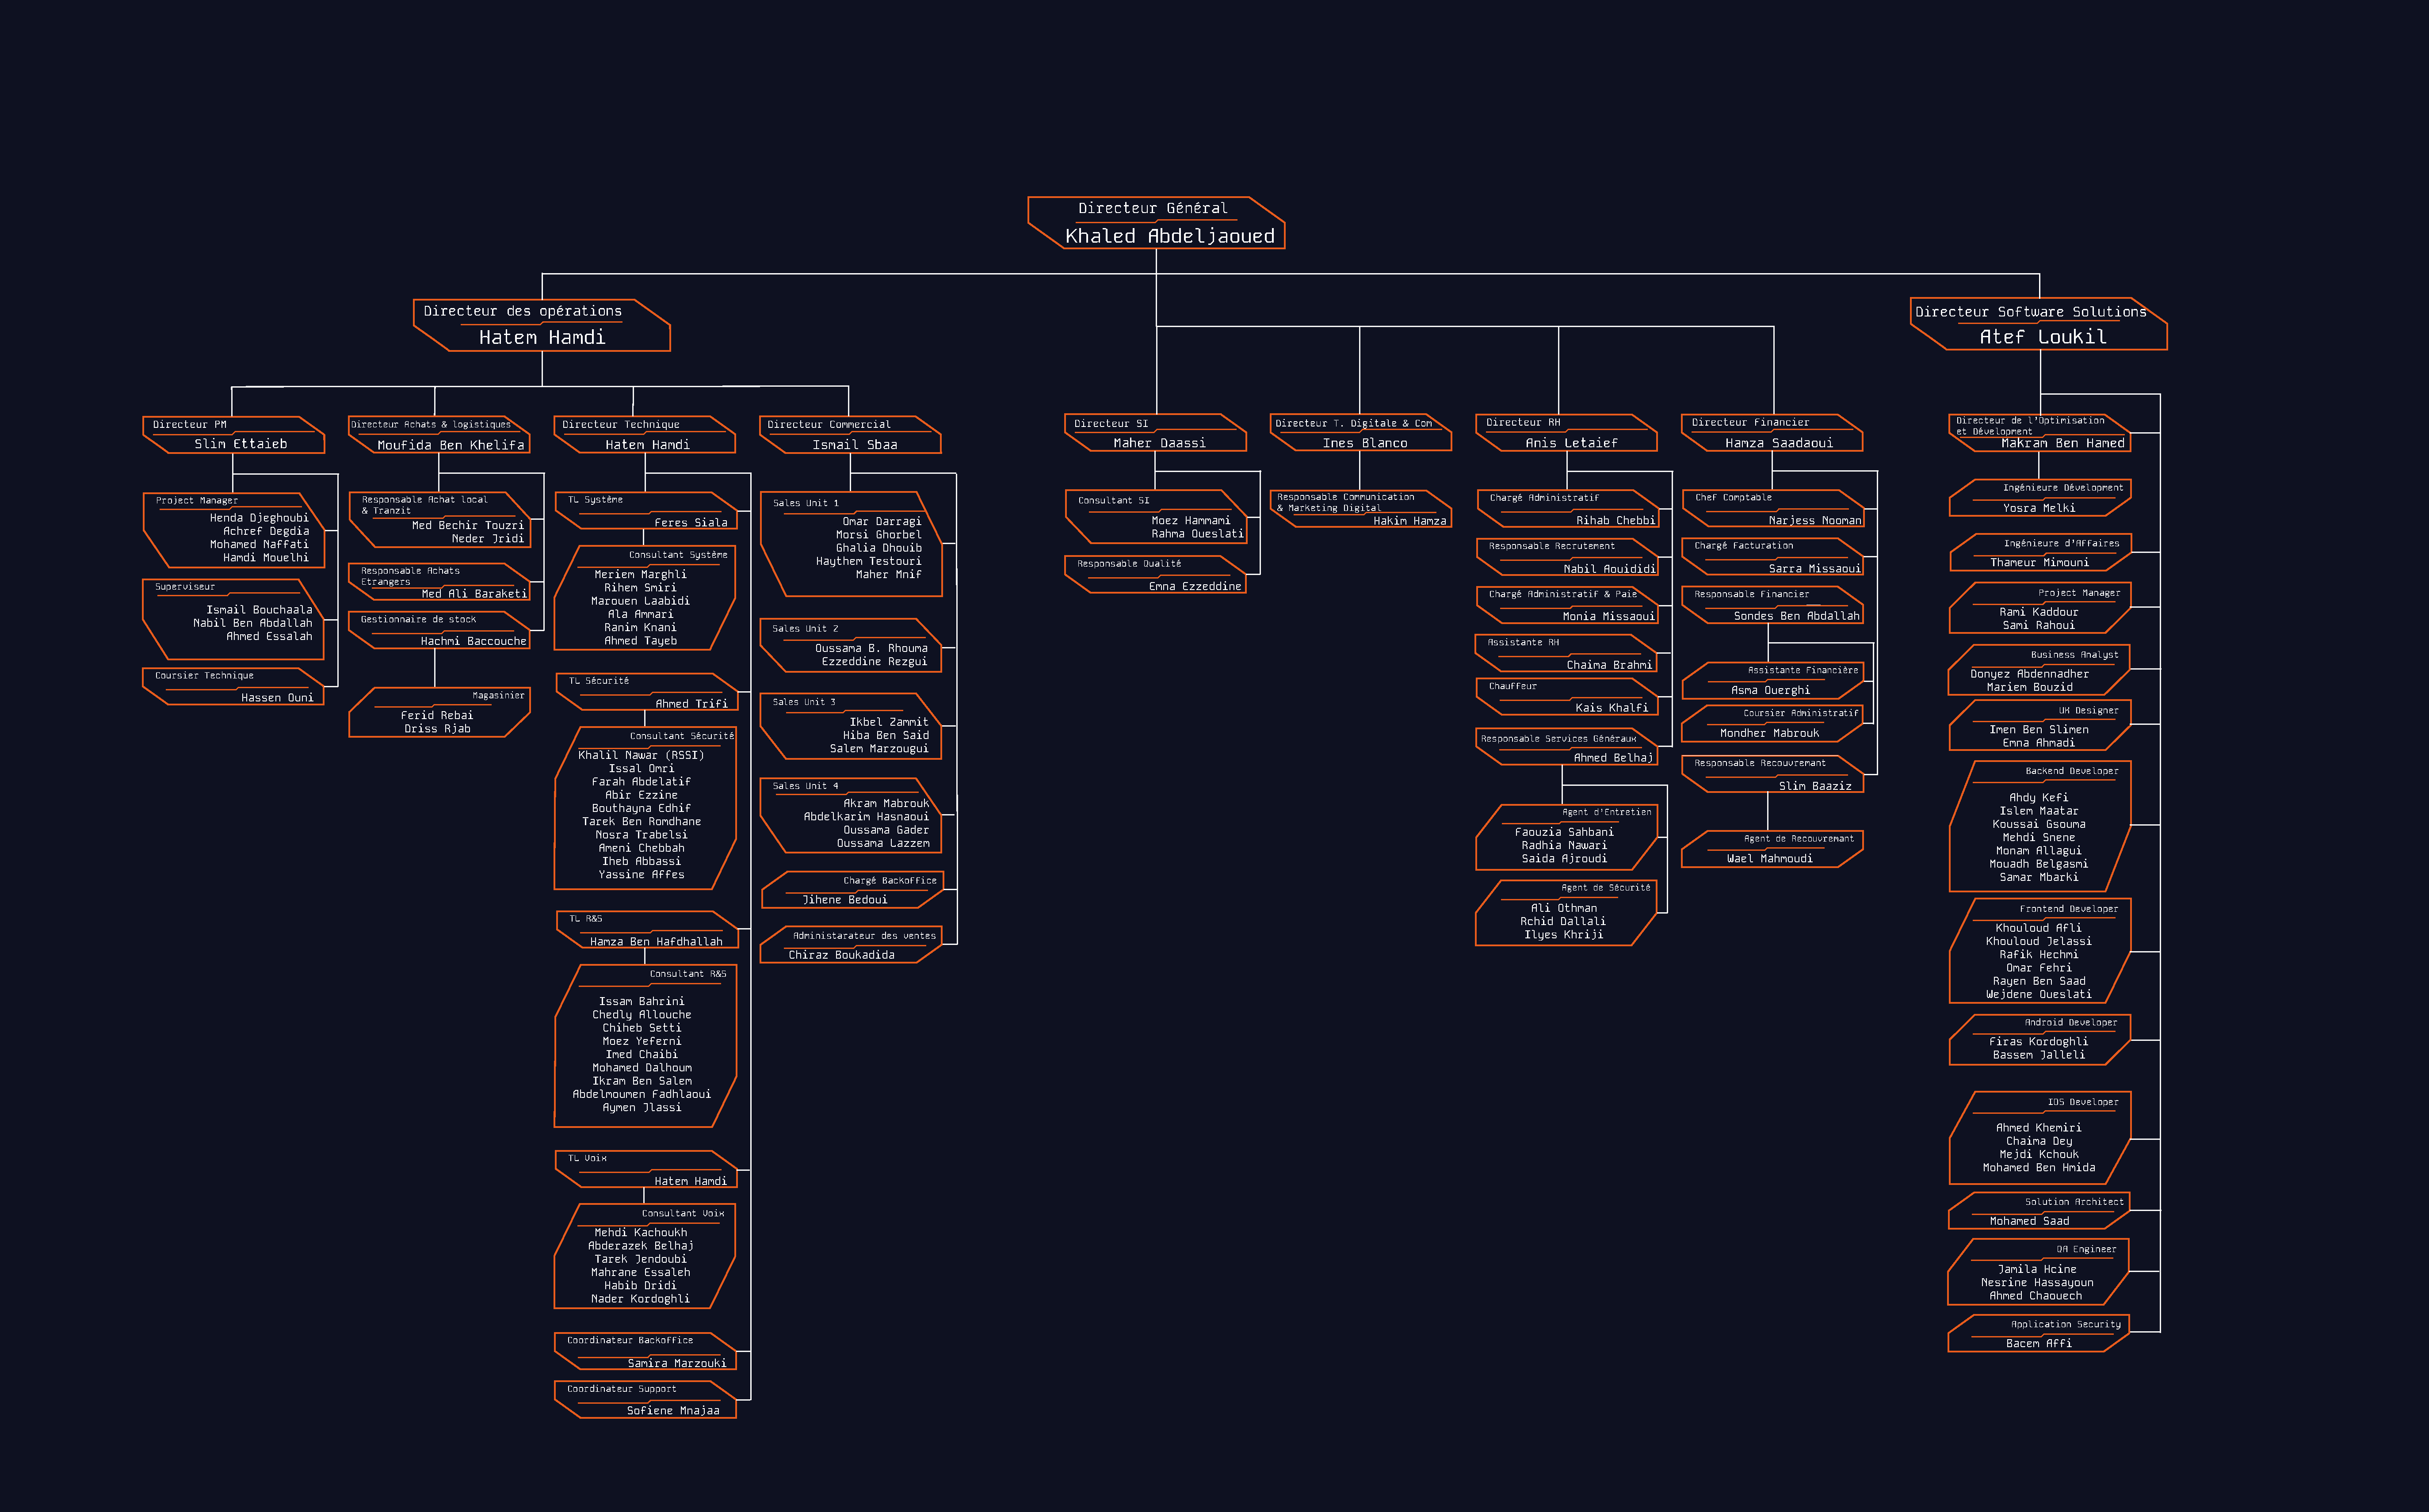
\includegraphics[width=\textwidth,height=0.88\textheight,keepaspectratio]{logos/organizational-chart.pdf}
	}{%
		\fbox{\parbox{0.96\textwidth}{
				\centering
				\vspace{4.0cm}
				\textit{Missing file: logos/organizational-chart.pdf}\\
				\textit{Place the organizational chart PDF in the logos folder to display it here.}
				\vspace{4.0cm}
		}}
	}
	\caption{Organizational chart: group management structure}
	\label{fig:group-management-structure}
\end{figure}
\clearpage

\subsection{Existing Information Systems}
At the time of the internship, the company relied on two separate information systems that supported different operational needs. Each system was useful in its own scope, but each one also represented only part of the information needed for complete attendance follow-up.

\textbf{BioTime} was the attendance-oriented system used in connection with the company's biometric device infrastructure. Its main role was to capture employee presence events such as check-in and check-out actions, together with timestamps and employee identifiers. In practice, this system provided the most direct view of physical presence at the office. From an HR perspective, BioTime was important because it produced the raw operational evidence used to verify punctuality, presence, and attendance history. However, by design, it focused mainly on biometric attendance events and did not explain why an employee might be absent from the office while still being officially active on external work.

Figure~\ref{fig:biotime-definition-placeholder} is reserved for an illustration of the BioTime software interface or architecture.

\begin{figure}[H]
	\centering
	\IfFileExists{assets/general/biotime-definition.jpg}{%
		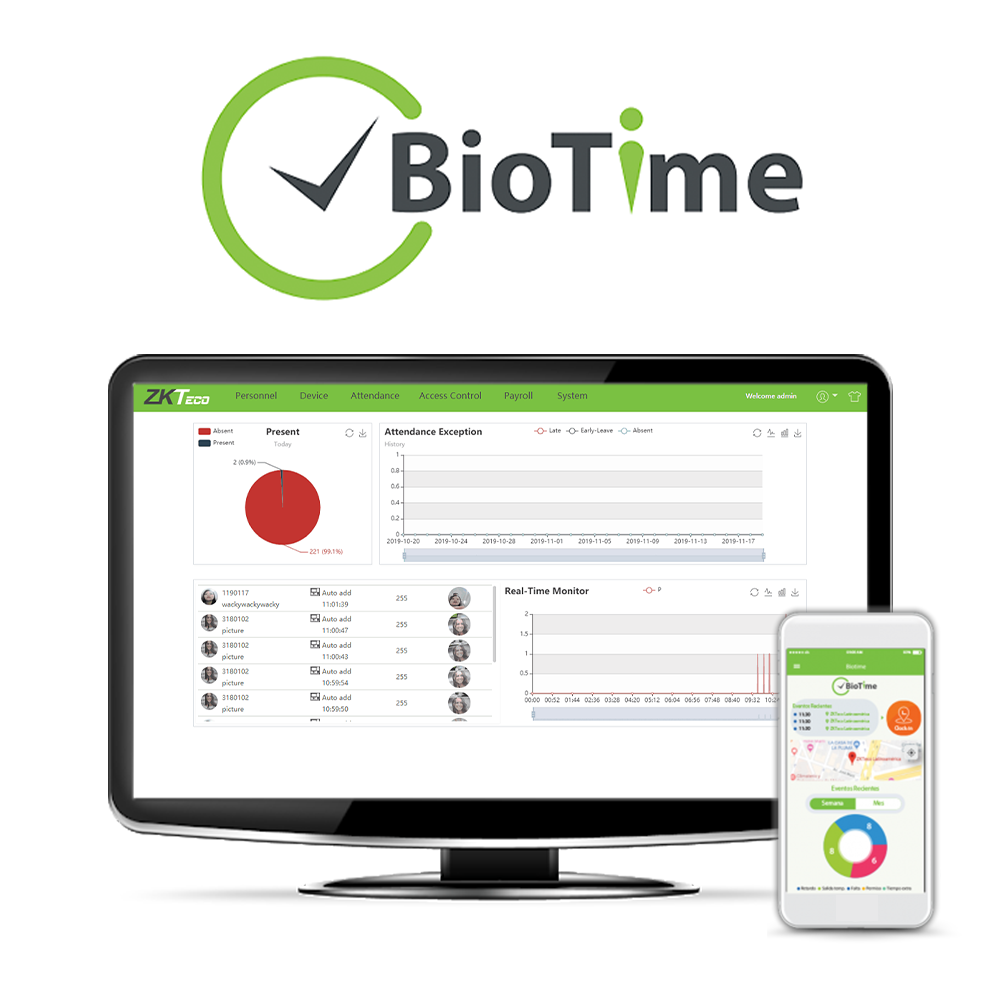
\includegraphics[width=0.90\textwidth,height=0.42\textheight,keepaspectratio]{assets/general/biotime-definition.jpg}
	}{%
		\fbox{\parbox{0.9\textwidth}{
				\centering
				\vspace{1.6cm}
				\textit{Missing file: assets/general/biotime-definition.jpg}\\
				\textit{Insert a BioTime software illustration, interface capture, or explanatory diagram.}
				\vspace{1.6cm}
		}}
	}
	\caption{Placeholder for BioTime software presentation}
	\label{fig:biotime-definition-placeholder}
\end{figure}

\textbf{EasyProject} was the project and HR-oriented system used to manage organizational and operational data beyond simple attendance events. It stored information related to employees, project assignments, organizational structure, schedules, and leave or mission context depending on the business workflow. This made EasyProject valuable for understanding the administrative and project-related explanation behind an employee's status. For example, when an employee was assigned to a mission, linked to a project, or covered by leave information, EasyProject could provide the context that BioTime alone could not show. As a result, it played a complementary role by describing the business meaning behind employee activity.

Figure~\ref{fig:easyproject-definition-placeholder} is reserved for an illustration of the EasyProject software interface or architecture.

\begin{figure}[H]
	\centering
	\IfFileExists{assets/general/easyproject-definition.jpg}{%
		
\includegraphics[width=0.90\textwidth,height=0.42\textheight,keepaspectratio]{assets/general/easyproject-definition.jpg}
	}{%
		\fbox{\parbox{0.9\textwidth}{
				\centering
				\vspace{1.6cm}
				\textit{Missing file: assets/general/easyproject-definition.jpg}\\
				\textit{Insert an EasyProject software illustration, interface capture, or explanatory diagram.}
				\vspace{1.6cm}
		}}
	}
	\caption{Placeholder for EasyProject software presentation}
	\label{fig:easyproject-definition-placeholder}
\end{figure}

In practice, these systems operated in isolation. BioTime described physical attendance, while EasyProject described organizational and project context. Since there was no native integration between them, overall visibility remained limited and data reconciliation had to be done manually.

\section{Problem Statement}
\subsection{Identified Pain Points}
Before this project began, the company already had two systems related to attendance follow-up, but each one reflected only part of the real situation.

\textbf{BioTime} is connected to the ZKTeco device installed at the company. It records clock-in and clock-out actions when employees are physically present at the office. \textbf{EasyProject}, on the other hand, is used for project follow-up and stores project-related information such as team members, assignments, and mission orders.

The main problem appeared when an employee was not physically present at the company because they were on an outside mission with a client. In such a case, the employee could be correctly registered in EasyProject as working on a specific mission or project, while no clock-in or clock-out record appeared in BioTime because the employee had not passed through the company device. For the HR department, this created a confusing situation: the employee seemed absent in BioTime but active in EasyProject.

Because of this separation, the company faced several operational difficulties:
\begin{itemize}[noitemsep]
	\item Attendance data was scattered between BioTime and EasyProject.
	\item The HR department had no unified view of the actual attendance status of employees.
	\item An employee could appear absent in one system while being active on a mission in the other.
	\item Reporting required manual verification and comparison between both systems.
	\item Manual reporting consumed time and increased the risk of errors.
	\item Managers and HR staff lacked a centralized tool for follow-up and decision-making.
\end{itemize}

\subsection{Project Objective}
The main objective of this internship project was to design a solution capable of bringing together BioTime and EasyProject within a centralized database and a unified application, mainly to simplify reporting for the HR department.

More specifically, the project aimed to:
\begin{itemize}[noitemsep]
	\item collect attendance data from BioTime and project-related mission data from EasyProject;
	\item integrate both data sources into a centralized PostgreSQL database through an ETL process;
	\item reconcile differences between physical office attendance and project mission activity;
	\item provide the HR department with a clearer and more reliable view of employee attendance;
	\item reduce manual reporting efforts and make follow-up faster and easier;
	\item provide secure, role-based access through a web application for Admin, HR, and Project Manager users.
\end{itemize}

\section{Requirements Analysis}
\subsection{Functional Requirements}

\textbf{Administrator}
\begin{itemize}[noitemsep]
	\item \textbf{FR-01}: Create and manage user accounts.
	\item \textbf{FR-02}: Assign roles (Admin, HR, Project Manager).
	\item \textbf{FR-03}: Assign projects to Project Managers.
	\item \textbf{FR-04}: Assign Project Managers to projects.
	\item \textbf{FR-05}: The Administrator shall not access employee details or attendance records.
\end{itemize}

\textbf{Human Resources (HR)}
\begin{itemize}[noitemsep]
	\item \textbf{FR-06}: View all employees across the organization.
	\item \textbf{FR-07}: View attendance records for all employees.
	\item \textbf{FR-08}: View attendance summaries and reports at global scope.
	\item \textbf{FR-09}: Manage HR attendance and leave follow-up operations.
\end{itemize}
\vspace{2cm}
\textbf{Project Manager}
\begin{itemize}[noitemsep]
	\item \textbf{FR-10}: View only projects assigned by the Administrator.
	\item \textbf{FR-11}: View members belonging to assigned projects.
	\item \textbf{FR-12}: View attendance records of members in assigned projects only.
\end{itemize}

\textbf{ETL \& System}
\begin{itemize}[noitemsep]
	\item \textbf{FR-13}: Extract attendance and HR data from BioTime and EasyProject on schedule.
	\item \textbf{FR-14}: Resolve duplicate records, ID mismatches, and timezone differences.
	\item \textbf{FR-15}: Store transformed and unified data in the main PostgreSQL database through \textbf{SQLAlchemy}.
	\item \textbf{FR-16}: Provide real-time synchronization capabilities.
\end{itemize}

\textbf{Dashboard \& Reporting}
\begin{itemize}[noitemsep]
	\item The dashboard shall display KPIs (present employees, absences, late arrivals, overtime).
	\item The system shall allow filtering by date range, project, and employee.
	\item Reports shall be exportable in standard formats.
\end{itemize}

\subsection{Non-Functional Requirements}
\begin{center}
	\renewcommand{\arraystretch}{1.2}
	\begin{tabular}{|l|l|>{\raggedright\arraybackslash}p{8cm}|}
		\hline
		\textbf{Category} & \textbf{Requirement ID} & \textbf{Description} \\
		\hline
		Performance & NFR-01 & API endpoints shall respond within 300ms for standard queries on datasets up to 5,000 employees. \\
		Security & NFR-02 & All API routes shall be protected by JWT-based authentication. Passwords shall be hashed using bcrypt. \\
		Security & NFR-03 & Role-based access control (RBAC) shall enforce permission boundaries. \\
		Reliability & NFR-04 & ETL shall handle source failures, log errors, and resume from the last successful sync point. \\
		Data Integrity & NFR-05 & Duplicate attendance records shall be prevented through ETL deduplication and unique constraints. \\
		Scalability & NFR-06 & The architecture shall support additional devices and new employee data sources. \\
		Usability & NFR-07 & The React interface shall be responsive on desktop and tablet screens. \\
		Maintainability & NFR-08 & Database migrations shall be managed with Alembic. \\
		Portability & NFR-09 & The application shall be Docker-compatible for deployment flexibility. \\
		\hline
	\end{tabular}
\end{center}

\section{Development Methodology: Scrum}
\subsection{Why Scrum Was Chosen}
Choosing the right development methodology was important for this project because the internship was short and the work included several parts at the same time. The project was not only about building one interface or one database. It also included system analysis, ETL design, backend development, frontend implementation, authentication, and RH Agent integration. Because of that, we needed a method that was organized but still flexible enough to adapt when needed.

For this reason, \textbf{Scrum} was the most suitable choice. It gave us a clear way to organize the work in small steps while still allowing changes and improvements during the internship.

\subsubsection{(a) Requirements were not fully clear from the start}
At the beginning of the project, the main objective was clear, but some details were still unknown. For example, the exact logic needed to reconcile BioTime attendance data with EasyProject mission data became clearer only after exploring the databases and testing different cases. In this kind of situation, Scrum is useful because it allows the solution to improve step by step instead of forcing everything to be fixed from the beginning.

\subsubsection{(b) The internship duration was limited}
The internship lasted about three months, so time management was very important. Scrum helped divide the work into short sprints, and each sprint produced a visible result. This made the progress easier to follow and helped keep the project moving in a structured way.

\subsubsection{(c) The project was divided into several parts}
The project naturally included several layers such as data exploration, ETL pipelines, database design, backend APIs, frontend modules, and agent integration. Scrum fit this structure well because each sprint could focus on one important part of the system while keeping the whole project connected.

\subsubsection{(d) Technical problems needed iterative work}
During the project, several technical issues appeared, such as missing identifiers, duplicated data, timestamp differences, and integration constraints between the two source systems. These issues could not always be solved directly in one attempt. Scrum was helpful because it allowed us to test, review, and improve the work from one sprint to another.

\subsubsection{(e) Scrum vs. Waterfall}
\textbf{Waterfall} is a more linear methodology. It usually starts with complete requirements, then moves step by step through analysis, design, implementation, and testing. This approach works well when the requirements are stable and well known from the beginning.

In our case, that was not really possible. Some requirements became clearer only during the work, especially after studying the source systems and starting implementation. If we had followed Waterfall, any change discovered later would have made the process heavier and less flexible.

Compared with Waterfall, Scrum was better for this project because:
\begin{itemize}[noitemsep]
	\item the requirements were still evolving;
	\item the project needed regular progress during a short internship;
	\item technical issues required continuous adjustment;
	\item working in small increments was more practical than following one rigid sequence.
\end{itemize}

\subsubsection{(f) Scrum vs. Kanban}
\textbf{Kanban} is also an agile method, but it focuses more on continuous task flow than on fixed sprints. It is very useful when work arrives continuously, like support or maintenance tasks.

In this project, the work followed a clearer progression from analysis to implementation, then to advanced modules and integration. Because of that, Scrum was more suitable than Kanban alone. Scrum gave us fixed periods with clear goals, which made it easier to organize the internship work and track results.

Compared with Kanban, Scrum was more adapted here because:
\begin{itemize}[noitemsep]
	\item it provided clear sprint objectives;
	\item it made milestone tracking easier;
	\item it helped structure the internship around deliverable results;
	\item it still kept enough flexibility to adjust the work when needed.
\end{itemize}

\subsubsection{(g) Final choice}
In the end, Scrum was chosen because it gave the best balance between structure and flexibility. It was organized enough to manage the project during a limited internship period, but also flexible enough to adapt to technical discoveries and requirement changes. That is why it was the most appropriate methodology for this project.

\subsection{Scrum Framework Overview}
\subsubsection{Roles}
\begin{itemize}[noitemsep]
	\item Product Owner: company supervisor.
	\item Scrum Master / Developer: intern.
\end{itemize}

\subsubsection{Artifacts}
\begin{itemize}[noitemsep]
	\item Product Backlog.
	\item Sprint Backlog.
	\item Increment.
\end{itemize}

\subsubsection{Ceremonies}
\begin{itemize}[noitemsep]
	\item Sprint Planning.
	\item Sprint Review.
	\item Sprint Retrospective.
\end{itemize}

\subsection{Sprint Plan}
\begin{center}
	\renewcommand{\arraystretch}{1.25}
	\setlength{\tabcolsep}{7pt}
	\begin{tabular}{|>{\centering\arraybackslash}m{1.8cm}|>{\centering\arraybackslash}m{3.1cm}|>{\raggedright\arraybackslash}p{8cm}|}
		\hline
		\rowcolor{gray!20}
		\textbf{Sprint} & \textbf{Duration} & \textbf{Main Objective} \\
		\hline
		Sprint 1 & Week 1 -- Week 2 & Chapter 2 --- System analysis and design: study the source systems, define the required data scope, and prepare the main conception artifacts. \\
		\hline
		Sprint 2 & Week 3 -- Week 4 & Chapter 3 --- ETL and unified database: implement the ETL pipelines and populate the centralized PostgreSQL database. \\
		\hline
		Sprint 3 & Week 5 -- Week 6 & Chapter 4 --- Authentication module: implement login, registration, administrator approval, and role-based access control. \\
		\hline
		Sprint 4 & Week 7 -- Week 8 & Chapter 5 --- Administration module: deliver user management, project assignment, and synchronization settings features. \\
		\hline
		Sprint 5 & Week 9 -- Week 10 & Chapter 6 --- HR functional modules: implement employee management, attendance follow-up, and leave handling interfaces. \\
		\hline
		Sprint 6 & Week 11 -- Week 12 & Chapter 7 --- Project Manager modules: deliver project, member, and attendance monitoring features for project managers. \\
		\hline
		Sprint 7 & Week 13 -- Week 14 & Chapter 8 --- RH Agent integration: integrate the RH Agent and finalize the intelligent assistance workflow. \\
		\hline
	\end{tabular}
\end{center}

\section{Chosen Technologies and Rationale}
To solve the integration problem between different systems while still building a maintainable full-stack solution, a focused technology stack was selected. This choice was guided by compatibility, reliability, development speed, and long-term maintainability.
\section{Technology Stack Table}
\renewcommand{\arraystretch}{1.1}
\footnotesize
\begin{center}
	\begin{tabular}{|>{\centering\arraybackslash}p{1.8cm}|>{\raggedright\arraybackslash}p{3.0cm}|>{\raggedright\arraybackslash}p{5.0cm}|>{\raggedright\arraybackslash}p{5.0cm}|}
		\hline
		\textbf{Icon} & \textbf{Technology} & \textbf{Description} & \textbf{Why I Chose It} \\
		\hline
		\TechIcon{logos/tech/sqlalchemy.pdf} & \textbf{SQLAlchemy} & Python ORM and SQL toolkit used in ETL and backend data access. & One clear way to work with both PostgreSQL and MySQL, which reduces complexity and repeated logic. \\
		\hline
		\TechIcon{logos/tech/fastapi.pdf} & \textbf{FastAPI} & Framework used to build REST APIs with validation and automatic documentation. & It allowed rapid API development with a clean structure and good performance. \\
		\hline
		{\scriptsize ALEMBIC} & \textbf{Alembic} & Tool used to manage and track database schema changes. & It keeps database changes clear, safe, and easy to track. \\
		\hline
		\TechIcon{logos/tech/postgresql.pdf} & \textbf{PostgreSQL} & Main unified relational database for transformed attendance and HR data. & Reliable, stable, and well suited for both daily operations and structured reporting. \\
		\hline
		\IfFileExists{logos/tech/redis.pdf}{\TechIcon{logos/tech/redis.pdf}}{\scriptsize REDIS} & \textbf{Redis} & In-memory data store used to speed up temporary data access and support fast backend operations. & Useful when low-latency access is needed for cached or short-lived data. \\
		\hline
		\TechIcon{logos/tech/mysql.pdf} & \textbf{MySQL (Source)} & Source database used by EasyProject and read by ETL jobs. & It let us integrate existing company data without changing the legacy system. \\
		\hline
		\TechIcon{logos/tech/resend.pdf} & \textbf{Resend} & Email delivery service for notifications and account communication. & Simple to use and reliable for sending account and notification emails. \\
		\hline
		\TechIcon{logos/tech/docker.pdf} & \textbf{Docker} & Platform used to package backend services and their dependencies. & It makes setup easier and keeps environments consistent. \\
		\hline
		\TechIcon{logos/tech/react.pdf} & \textbf{React} & Frontend library used to build dynamic interfaces with reusable components. & It made the interface easier to organize and reuse. \\
		\hline
	\end{tabular}
\end{center}

\vspace{0.4cm}

\begin{center}
	\begin{tabular}{|>{\centering\arraybackslash}p{1.8cm}|>{\raggedright\arraybackslash}p{3.0cm}|>{\raggedright\arraybackslash}p{5.0cm}|>{\raggedright\arraybackslash}p{5.0cm}|}
		\hline
		\textbf{Icon} & \textbf{Technology} & \textbf{Description} & \textbf{Why I Chose It} \\
		\hline
		\TechIcon{logos/tech/tailwindcss.pdf} & \textbf{Tailwind CSS} & CSS framework used to style the interface quickly. & It helped us build pages faster with a more consistent design. \\
		\hline
		\TechIcon{logos/tech/shadcn-ui.pdf} & \textbf{shadcn/ui} & Reusable UI components built on top of Radix and Tailwind. & It helped us create clean interfaces faster while keeping flexibility. \\
		\hline
		\TechIcon{logos/tech/tanstack.pdf} & \textbf{TanStack Table} & Table library used for sorting, filtering, and pagination. & It was very useful for large employee and attendance tables. \\
		\hline
		\TechIcon{logos/tech/tanstack.pdf} & \textbf{TanStack Query} & Library used for API state management and caching. & It improved performance and made async data handling cleaner. \\
		\hline
		\TechIcon{logos/tech/langgraph.pdf} & \textbf{LangGraph} & Framework used to build stateful, multi-step LLM workflows and agent graphs. & It was useful for organizing the RH Agent flow in a controlled way. \\
		\hline
		\TechIcon{logos/tech/langchain.pdf} & \textbf{LangChain} & Framework used for prompt chaining, tool use, and retrieval integration. & It made AI feature integration faster and easier. \\
		\hline
		\TechIcon{logos/tech/ollama.pdf} & \textbf{Ollama} & Local runtime used to serve open-source language models on private infrastructure. & It allowed private AI inference that fits company data-security needs. \\
		\hline
		\IfFileExists{logos/tech/vscode.pdf}{\TechIcon{logos/tech/vscode.pdf}}{\scriptsize VS CODE} & \textbf{VS Code} & Lightweight and extensible editor used for frontend and backend development. & It gave a fast editing experience with many useful extensions. \\
		\hline
		\IfFileExists{logos/tech/pycharm.pdf}{\TechIcon{logos/tech/pycharm.pdf}}{\scriptsize PYCHARM} & \textbf{PyCharm} & Python IDE used for backend and ETL development. & It made Python development easier with good debugging and code tools. \\
		\hline
		\IfFileExists{logos/tech/git.pdf}{\TechIcon{logos/tech/git.pdf}}{\scriptsize GIT} & \textbf{Git} & Version control system used to track and manage source code changes. & It made collaboration and sprint work safer and easier to manage. \\
		\hline
		\IfFileExists{logos/tech/github.pdf}{\TechIcon{logos/tech/github.pdf}}{\scriptsize GITHUB} & \textbf{GitHub} & Remote repository hosting and collaboration platform built around Git. & It helped the team share code, review changes, and stay organized. \\
		\hline
	\end{tabular}
\end{center}
\normalsize

Overall, this stack helped address the main project challenge: connecting two separate source systems, exposing secure and maintainable APIs, and building a responsive interface for day-to-day follow-up.

\section{Chapter Conclusion}
This chapter established the foundation of the project by presenting the organizational context and the main challenge created by the coexistence of two isolated systems: BioTime and EasyProject.

The proposed response is a unified architecture built around an ETL pipeline, a consolidated PostgreSQL database, a FastAPI backend, and a React web dashboard designed to ensure reliable and conflict-free attendance monitoring.

